\section{Mathematics, Physics, and Statistical Methods}

\subsection{Mathematics}

\subsubsection{Gaussian Distribution}

The probability density function of Gaussian distribution is as follows, where $\mu$ is the mean and $\sigma$ is the standard deviation.

\begin{equation}
    \mathrm{N}(\mu, \sigma^2): \quad \frac{1}{\sigma\sqrt{2\pi}} \exp{\left(-\frac{(x - \mu)^2}{2 \sigma^2} \right)}
\end{equation}

So, we can see that the log of that is a quadratic function.

\begin{equation}
    \ln{P(x)} = -\frac{(x - \mu)^2}{2 \sigma^2} - \ln{\sigma} - \frac{1}{2} \ln{2\pi}
\end{equation}

For more information, please move into \href{https://en.wikipedia.org/wiki/Normal_distribution}{Wikipedia: Normal Distribution}.

\subsubsection{Chi Distribution}

The chi distribution is a probability distribution with positive real numbers as its domain. We have to distinguish between this and the chi-square distribution.

When $k$ variables $x_k$ have a standard normal distribution, we define that the following value $y$ has a $k$-degree chi distribution.

\begin{equation}
    y = \sqrt{\sum_{i=1}^k x_i^{\ 2}}
\end{equation}

Two famous examples are the Rayleigh distribution as a 2-degree chi distribution and the Maxwell-Boltzmann distribution as a 3-degree chi distribution.

The probability density distribution is as follows.

\begin{figure}[h]
\centering
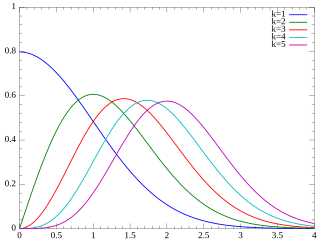
\includegraphics[width=0.5\textwidth]{figs/chi.png}
\caption{The probability density function of chi-distribution.}
\end{figure}

\begin{equation}
    f(x;k) = \frac{x^{k-1} e^{-x^2/2}}{2^{(k/2) - 1} \Gamma(k/2)} \quad (x>0)
\end{equation}

For more information such as cumulative distribution function, visit \href{https://en.wikipedia.org/wiki/Chi_distribution}{Wikipedia: Chi Distribution}.

\subsubsection{Spherical Coordinate System}

To exhibit an isotropic distribution, an understanding of the spherical coordinate system is required.

\begin{figure}[h]
\centering
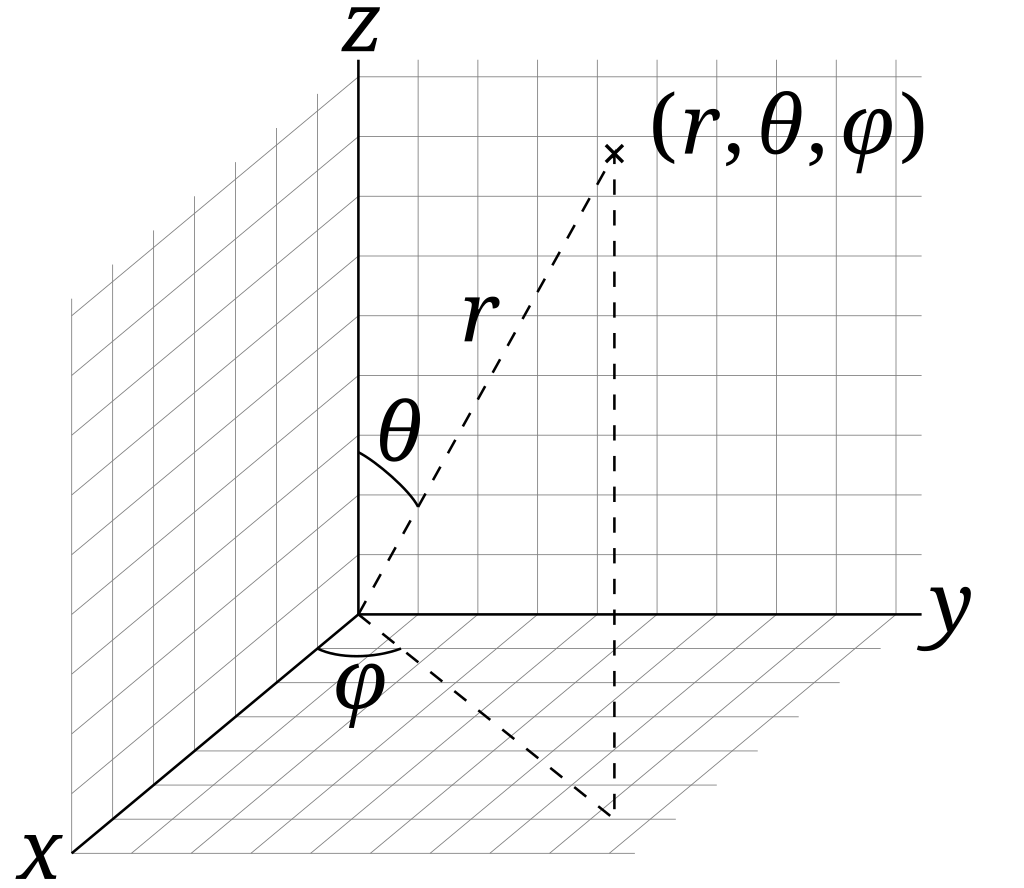
\includegraphics[width=0.5\textwidth]{figs/sphe.png}
\caption{Spherical Coordinate.}
\end{figure}

We define the origin as $O$, the point we think as $P$, and the projection of $P$ to $xy$-plane as $P'$.

The variables are as follows.

$r$: Radius, Distance from coordinate origin ($r \geq 0$)

$\theta$: Inclination, Angle from the direction $+z$ to the line $OP$ ($0 \leq \theta \leq \pi$)

$\varphi$: Azimuth, Angle from the direction $+x$ to the line $OP'$ ($0 \leq \theta < 2\pi$)

In the integration of orthogonal and spherical coordinates, the relationship follows.

\begin{equation}\label{int}
    \int dV = \int d^3 \mathbf{x} = \int_0^\infty dr \int_0^\pi r d\theta \int_0^{2\pi} r \sin{\theta} d\varphi
\end{equation}

Let us assume that events occur isotropically and the inclination angle is $\theta \sim \theta + d \theta$. Of course, the radius and azimuth angle have any possible value.

Given $\theta$, the number of events is proportional to $\sin{\theta}$(Sine distribution). It is easy to see by referring to equation (\ref{int}).

For more information such as coordinate conversion, differentiation or integration, visit \href{https://en.wikipedia.org/wiki/Spherical_coordinate_system}{Wikipedia: Spherical Coordinate System} or read \textit{Arfken and Weber, 7th edition}.

\subsubsection{Fourier Transformation}

Fourier transform is a transformation that decomposes a function over time or space into frequency components. The definition is as follows.

\begin{equation}
    \hat{h}(f) = \int_{-\infty}^\infty dt \ h(t)e^{-2\pi i f t}
\end{equation}

Note that the output of the Fourier transform is a complex domain of frequency, not a real number domain.

The Fourier inverse transformation is defined as follows.

\begin{equation}
    h(t) = \int_{-\infty}^\infty dt \ \hat{h}(f)e^{2\pi i f t}
\end{equation}

The Fourier transform is represented by the letter $\mathcal{F}$.

Depending on the literature or Python packages, the proportional constant may be multiplied during Fourier transform/inverse transform, so check it carefully.

The following basic properties are established in Fourier transform.

\begin{align}
    &ah(x) + bg(x) \overset{\mathcal{F}}{\iff} a\hat{h}(f) + b\hat{g}(f) & \text{linearity} \\
    &h(t - t_0) \overset{\mathcal{F}}{\iff} e^{-2\pi i f t} \hat{h} (f) & \text{time-shift} \\
    &e^{2\pi i f_0 t}h(t) \overset{\mathcal{F}}{\iff} \hat{h} (f - f_0) & \text{frequency-shift} \\
    &h(at) \overset{\mathcal{F}}{\iff} \frac{1}{|a|} \hat{h} \left( \frac{f}{a} \right) & \text{time-scaling}
\end{align}

The conversion theorem is as follows.

\begin{equation}
    (g*h)(t) \equiv \int_{-\infty}^\infty g(\tau) h(t - \tau) \ d \tau \overset{\mathcal{F}}{\iff} \hat{g}(f) \hat{h}(f)
\end{equation}

Some important Fourier transformations are as follows.

\begin{align}
    &1 \overset{\mathcal{F}}{\iff} \delta(f) \\
    &\delta(t) \overset{\mathcal{F}}{\iff} 1 \\
    &e^{iax} \overset{\mathcal{F}}{\iff} \delta \left(f - \frac{a}{2\pi} \right)
\end{align}

Fourier transform is used in various fields such as solving linear differential equations, quantum mechanics, signal processing, and analysis.

For more information such as the applications, Fourier transform tables, etc., visit \href{https://en.wikipedia.org/wiki/Fourier_transform}{Wikipedia: Fourier Transformation}.

\subsection{Physics}

\subsubsection{Chirp Mass}

The chirp mass(In the 2-body system) determines the leading-order orbital evolution of the system as a result of energy loss from emitting gravitational waves.(\href{https://en.wikipedia.org/wiki/Chirp_mass}{Wikipedia: Chirp Mass})

We can define the chirp mass as

\begin{equation}
    \mathcal{M} = \frac{(m_1 m_2)^{3/5}}{(m_1 + m_2)^{1/5}} = \mu^{3/5} M^{2/5}
\end{equation}

Where

\begin{equation}
    M = m_1 + m_2, \quad \mu = \frac{m_1 m_2}{m_1 + m_2}
\end{equation}

The frequency of the gravitational wave (generated by the binary orbit) evolves using the chirp mass,

\begin{equation}
    \dot{f} = \frac{96}{5} \pi^{\frac{8}{3}} \left( \frac{G \mathcal{M}}{c^3} \right)^{\frac{5}{3}} f^{\frac{11}{3}}
\end{equation}

So we can know the chirp mass as

\begin{equation}
    \mathcal{M} = \frac{c^3}{G} \left( \frac{5}{96} \pi^{-\frac{8}{3}} f^{-\frac{11}{3}} \dot{f} \right)^{\frac{3}{5}}
\end{equation}

For more information, visit \href{https://en.wikipedia.org/wiki/Chirp_mass}{Wikipedia: Chirp Mass}.

\subsubsection{Polarizations of Gravitational Waves}

There are two polarizations (plus, cross) in gravitational waves.

\begin{example}
Let's consider the following metric perturbations.

\begin{equation}
    g_{\mu \nu} = \eta_{\mu \nu} + h_{\mu \nu}, \quad h \equiv \eta^{\mu \nu}h_{\mu \nu}
\end{equation}

The plane wave solutions of gravitational waves (in the general relativity) traveling in the positive $z$-direction satisfy the following.

\begin{equation}
    \bar{h}_{\mu \nu} \equiv h_{\mu \nu} - \frac{1}{2} h, \quad \square \bar{h}_{\mu \nu} = 0 
\end{equation}

If you think about it in the same way you learn from electro-magnetics, these positive z-direction plane waves have two polarizations. This solution defines the following TT gauge(Transverse-traceless gauge).

\begin{equation}
    h_{ab}^{\mathrm{TT}}(t,z) = \begin{pmatrix} h_+ & h_\times \\ h_\times & -h_+ \end{pmatrix} \cos{[\omega(t-z/c)]}
\end{equation}

This gravitational wave acts on the interval $ds^2$ as follows.

\begin{align}
    \nonumber ds^2 = &-c^2 dt^2 + dz^2 + \{ 1 + h_+ \cos{[\omega(t-z/c)]}\} dx^2 \\
    &\quad + \{ 1 - h_+ \cos{[\omega(t-z/c)]} \} dy^2 + 2h_\times \cos{[\omega(t-z/c)]} dxdy
\end{align}

Here I only listed the results, and see pages 3 to 9 of \textit{Maggiore} (2008) for a detailed explanation.
\end{example}

\begin{figure}[h]
\centering
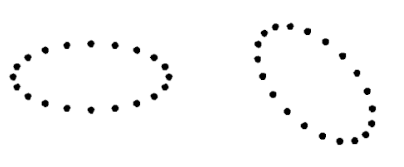
\includegraphics[width=0.5\textwidth]{figs/pol.png}
\caption{The plus(left) and cross(right)-polarizations of the gravitational waves.}
\end{figure}

The gravitational wave can have more polarizations (if we don't assume that the general relativity is correct), but this is not covered here.

\subsubsection{Waveform of Gravitational Waves}

Before two large objects (such as black holes) collide with each other, they have time to orbit. At this time, energy is released in the form of gravitational waves. Initially, low frequencies and low amplitude gravitational waves occur. And as the two objects continue to revolve and get closer to each other, their frequencies and amplitudes increase. Eventually, when the two objects approach a certain level or higher, the frequencies and amplitude increase dramatically.

Here is the waveform of the GW150914, which is the first detected gravitational-wave signal.

\begin{figure}[h]
\centering
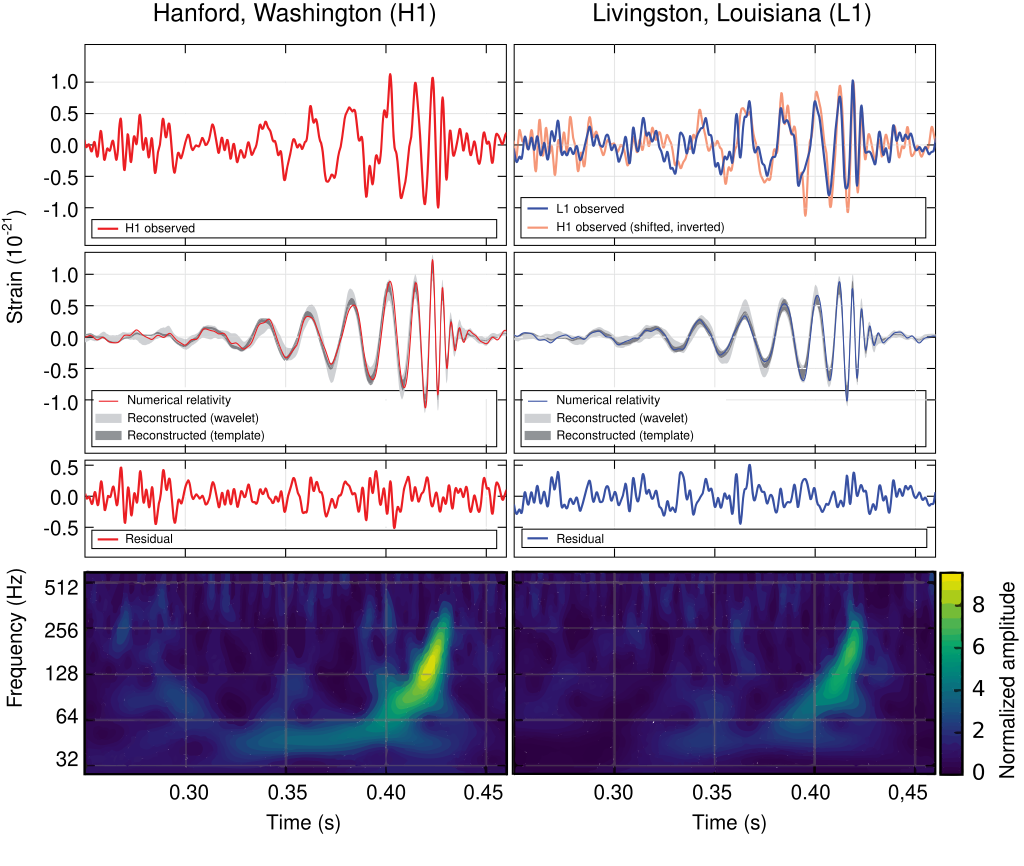
\includegraphics[width=0.7\textwidth]{figs/150914.png}
\caption{The waveform of GW150914. Figure from \href{https://en.wikipedia.org/wiki/First_observation_of_gravitational_waves}{Wikipedia: First Observation of Gravitational Waves}}
\end{figure}

Let's assume that two massive objects are orbiting each other in a circular orbit.

We define as $t_{\mathrm{ret}} = t - r/c$ (when the gravitational wave waveform we observe occurs) and $f$ as the frequency of the gravitational wave. $\theta$ is the angle between the observer and the straight line connecting the gravitational source and the axis of rotation of the gravitational source celestial body (the co-latitude) and $\phi$ is the phase.

And then we can estimate the waveform of the gravitational-wave.

\begin{align}
    h_+(t) &= \frac{4}{r} \left( \frac{G\mathcal{M}}{c^2} \right)^{\frac{5}{3}} \left( \frac{\pi f}{c} \right)^{\frac{2}{3}} \frac{1 + \cos^2{\theta}}{2} \cos{(2\pi f t_{\mathrm{ret}} + 2 \phi)} \\
    h_\times(t) &= \frac{4}{r} \left( \frac{G\mathcal{M}}{c^2} \right)^{\frac{5}{3}} \left( \frac{\pi f}{c} \right)^{\frac{2}{3}} \cos{\theta} \sin{(2\pi f t_{\mathrm{ret}} + 2 \phi)}
\end{align}

For more information such as the derivation of the formula, see \textit{Maggiore}(2008) Sec. 3 and 4.

\subsubsection{The Time to Coalescence}

About elliptical orbit, let's think that we have the samimajor axis $a_0$, the eccentricity $e_0$ and the orbital period $T_0$. The subscript $0$ means that they are initial value. And $M = m_1 + m_2$ is the total mass, $\mu$ is the reduced mass.

We can see the orbital period from the fact that the gravitational wave frequency $f$ is twice the orbital frequency.

We have the coalescence time $\tau_0$ as

\begin{align}
    \tau_0(a_0, e_0) &\simeq 9.829\mathrm{Myr} \left( \frac{T_0}{1\mathrm{hr}} \right)^{\frac{8}{3}} \left( \frac{M_\odot}{M} \right)^{\frac{2}{3}} \left( \frac{M_\odot}{\mu} \right) f(e_0) \\
    F(e_0) &= \frac{48}{19} \frac{1}{[g(e_0)]^4} \int_{0}^{e_0} de \ \frac{[g(e)]^4 (1 - e^2)^{5/2}}{e(1 + \frac{121}{304} e^2)} \simeq \frac{768}{429} (1 - e_0^{\ 2})^\frac{7}{2} \\
    g(e) &= \frac{e^{12/19}}{1 - e^2} \left( 1 + \frac{121}{304} e^2 \right)^\frac{870}{2299}
\end{align}

For circular orbit case, because eccentricity $e_0$ is 0, so the coalescence time $\tau_0$ is

\begin{equation}
    \tau_0 \simeq 9.829\mathrm{Myr} \left( \frac{T_0}{1\mathrm{hr}} \right)^{\frac{8}{3}} \left( \frac{M_\odot}{M} \right)^{\frac{2}{3}} \left( \frac{M_\odot}{\mu} \right)
\end{equation}

For more information such as the derivation of the formula, see \textit{Maggiore}(2008) from Sec. 4.1.1 to 4.1.3.

\subsubsection{Gravitational Lens}

\subsubsection{Signal}

The time-domain signal-strain-data we can see from the detector is expressed as a linear combination of $h_+$ and $h_\times$.

\begin{equation}
    h(t) = F_+(\hat{\mathbf{n}}) h_+(t) + F_\times (\hat{\mathbf{n}}) h_\times (t)
\end{equation}

Where $\hat{\mathbf{n}}$ is the direction vector. This is determined from polarization and azimuth. For more information, see \textit{Maggiore}(2008) Sec. 7.2.

The Python package Pycbc has a function of entering hplus, hcross, polarization, and azimuth to project it. For more information about this, see \href{https://pycbc.org/pycbc/latest/html/waveform.html}{Pycbc Waveform Documents}.

\subsubsection{Signal and Noise}

When detecting gravitational waves, the amplitude of noise is greater than that of ordinary signals. Therefore, it is necessary to identify the frequency characteristics of the signal in noise by Fourier transforming them.

[Physical part: formula]

\subsubsection{Detection Analysis}

\subsubsection{Interferometers}

\subsection{Statistical Methods}

\subsubsection{Bayes Theorem}

Given two probability distributions and conditional probabilities, the probability of two occurring simultaneously is as follows.

\begin{equation}
    P(A \cup B) = P(A|B) P(B) = P(B|A) P(A)
\end{equation}

Bayes' theorem is a way to find a conditional probability $P(B|A)$ when you know a conditional probability $P(A|B)$. The formula is as follows.

\begin{equation}
    P(B|A) = \frac{P(A|B)P(B)}{P(A)}
\end{equation}

The general formula is as follows.

\begin{equation}\label{mlm}
    P(x_0|A) = \frac{P(x_0) P(A|x_0)}{P(A)} = \frac{P(x_0) P(A|x_0)}{\int dx \ P(x) P(A|x)}
\end{equation}

For more information such as application example, visit \href{https://en.wikipedia.org/wiki/Bayes%27_theorem}{Wikipedia: Bayes Theorem}.

\subsubsection{Maximum Likelihood Method}

The likelihood is a probability known empirically beforehand. By formula(\ref{mlm}), we define the likelihood $\mathcal{L}$ as follows.

\begin{equation}
    \mathcal{L}(A|x) = P(x|A)
\end{equation}

Here, $A$ is the surrounding environment (parameters, such as the mass of the black holes, the distance from observer, etc.) that produces the result value, and $x$ is the result value. We know the result($x$) from observations, and we need to find the surrounding environment($A$) that produces the result.

Let the parameters such that the probability distribution $P(x|A)$ is maximized be called the estimated value $A_0$. In this case, we can estimate that the observation value $x$ is more likely to be generated by parameter $A_0$ compared to other parameters.

Therefore, when $x$ is fixed, we need to find $A$ so that the likelihood has an extreme value.

\begin{equation}
    A_0 = \underset{A}{\arg\max} \ {\mathcal{L}(A|x)}
\end{equation}

We can obtain parameters that derive the maximum likelihood in the preferred method of the two. (the latter is usually preferred here)

\begin{subequations}
    \begin{align}
        0 &= \frac{\partial{\mathcal{L}(A|x)}}{\partial A} \\
        0 &= \frac{\partial{\ln{\mathcal{L}(A|x)}}}{\partial A}
    \end{align}
\end{subequations}

For a thorough mathematical description or an explanation of an algorithm, etc., visit \href{https://en.wikipedia.org/wiki/Maximum_likelihood_estimation}{Wikipedia: Maximum Likelihood Estimation}.

\subsubsection{Metropolis-Hastings Method}

Markov Chain Monte Carlo(MCMC) method is an example of rejection method. In this method, we need a probability distribution(it is OK if not-renormalized).

Metropolis-Hastings method is one of the examples of MCMC. In this method, we need a probability distribution and a proposal distribution. Here I explain the algorithm only, not proof.\footnote{The notation and explanation are based on Okubo(2022), https://github.com/compsci-alliance/many-body-problems}\footnote{The proof is in Chib \& Greenberg(1995).}

The set of all states is $\{ \Gamma \}$. We have a probability distribution $P(\Gamma)$ and a proposal distribution $q(\Gamma | \Gamma')$,

Step 0: Prepare an initial state $\Gamma_0 \in \{ \Gamma \}$

\quad loop $t$

\qquad 1. Make next candidate state $\Gamma'$ randomly from the proposal distribution $q(\Gamma' | \Gamma_t)$

\qquad 2. Make a uniform random number $r \in [0,1]$

\qquad 3. Select the next state $\Gamma_{t + 1}$ based on $r$ as

\begin{equation}
    \Gamma_{t+1} = \begin{cases} \Gamma' & (r \leq a (\Gamma_t \to \Gamma') \\ \Gamma_t & (\mathrm{else}) \end{cases}
\end{equation}

Where the acceptance probability is as follows.

\begin{equation}
    a (\Gamma_t \to \Gamma') = \min{\left(1, \ \frac{P(\Gamma') q(\Gamma_t | \Gamma')}{P(\Gamma_t) q(\Gamma' | \Gamma_t)} \right)}
\end{equation}

The example problem is as follows.

\begin{example}

The probability density function is as follows.

\begin{equation}
    p(x) = 0.3 \frac{1}{2 \sqrt{2\pi}} \exp{\left(- \frac{(x + 5)^2}{8} \right)} + 0.7 \frac{1}{\sqrt{2\pi}} \exp{\left(- \frac{(x - 3)^2}{2} \right)}
\end{equation}

The proposal density funcion is a normal distribution function, as follows.

\begin{equation}
    q(x^* | x) = \frac{1}{10\sqrt{2\pi}} \exp{\left( -\frac{(x^* - x)^2}{200} \right)}
\end{equation}

Set initial state as random normal distribution with mean 0 and standard deviation 10. The probability density is as follows.

\begin{equation}
    p_0 (x_0) = \frac{1}{10\sqrt{2\pi}} \exp{\left( -\frac{x_0^{\ 2}}{200} \right)}
\end{equation}

Calculate the logarithm of the acceptance rate.

\begin{equation}
    \ln{a} = \ln{p(x^*)} - \ln{p(x_{t-1})} + \ln{q(x_{t-1} | x^*)} - \ln{q(x^* | x_{t-1})}
\end{equation}

Make a random $r$ from $(0,1]$ and compare $r$ and the acceptance rate.

\begin{align}
    \ln{\alpha} &= \min{(0, \ln{a})} \\
    \ln{r} \leq \ln{a} &\to x_{t} = x^* \\
    \ln{r} > \ln{a} &\to x_{t} = x_{t-1}
\end{align}

Repeat this 5000 times($t = 5000$).

The code is as follows.

\begin{python}[Python3]
import numpy as np
import math
import scipy.stats as stats
import matplotlib.pyplot as plt
def p(x):
    return 0.3 * (2 * math.sqrt(2 * math.pi)) ** (-1) * np.exp(-(x + 5) ** 2 / 8) + 0.7 * (math.sqrt(2 * math.pi)) ** (-1) * np.exp(-(x - 3) ** 2 / 2)
def logp(x):
    return np.log(p(x))
T = 5000
sigma = 10
for i in range(1, T+1):
    candidate = np.random.normal(size = 1, loc=learn[i-1], scale=sigma)
    loga = logp(candidate) - logp(learn[i-1]) + stats.norm(candidate, sigma).logpdf(learn[i-1]) - stats.norm(learn[i-1], sigma).logpdf(candidate)
    logalpha = min(0, loga)
    r = np.random.uniform(size=1)
    logr = math.log(r)
    if logr <= logalpha:
        learn = np.append(learn, candidate)
    else:
        learn = np.append(learn, learn[i-1])
grid = np.arange(-10, 10, 0.01)
plt.plot(grid, p(grid))
plt.hist(learn, bins = 40, density = True)
plt.show()
\end{python}

The result is as follows.

\begin{figure}[h]
\centering
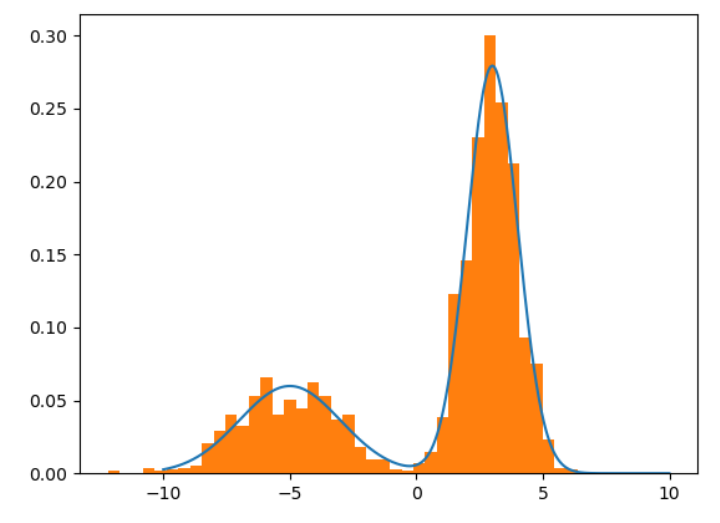
\includegraphics[width=0.5\textwidth]{figs/met.png}
\caption{Metropolis-Hastings example code result}
\end{figure}

\end{example}

This part deals with similar content as \href{https://en.wikipedia.org/wiki/Metropolis%E2%80%93Hastings_algorithm}{Wikipedia: Metropolis-Hastings Algorithm}, so you can read and compare them.

\subsubsection{Inverse Transform Method}

When we have a probability distribution $p(x)$, we can make a simulation program to generate that distribution.

The cumulative probability distribution $P(x)$ is as follows.

\begin{equation}
    P(x) = \int_{-\infty}^x p(x) \ dx
\end{equation}

Let's think about the slope of $P(x)$. This is a probability distribution $p(x)$.

\begin{align}
    y &\equiv P(x) \\
    dy &= p(x)dx
\end{align}

Therefore, we can know that $dy$ is proportional to the probability distribution. What that does mean?

Let us generate random numbers $y$ that have uniform distribution in the rages of $[0,1]$. If we choose a specific $y_0 \sim y_0 + dy$, we can get the number of $y$ such that $y_0 \leq y \leq y_0 + dy$. The number is proportional to $p(x)$.

\begin{equation}
    dy = p(x)dx \propto p(P^{-1}(y))
\end{equation}

Therefore, we can correspond y to x, as follows.

\begin{equation}
    x = P^{-1}(y)
\end{equation}

So the $x$ have the probability distribution $p(x)$.

I think the explanation might be difficult to understand, so let's see an example.

\begin{example}

The range of inclination angle in GWpy package is $-\pi/2 \leq \theta \leq \pi/2$, so if we want the isotropic spherical distribution, we should use cosine distribution rather than sine distribution. See equation (\ref{int}).

The distribution is as follows.

\begin{align}
    p(x) &= \begin{cases} \frac{1}{2} \cos{x} & ( -\pi/2 \leq x \leq \pi/2) \\ 0 & (\mathrm{else}) \end{cases} \\
    P(x) &= \begin{cases} 0 & (x \leq -\pi/2 ) \\ \frac{1}{2} \sin{x} + \frac{1}{2} & ( -\pi/2 \leq x \leq \pi/2) \\ 1 & (x \geq \pi/2 ) \end{cases} \\
    x &= P^{-1} (y) = \arcsin{(2y - 1)} \quad (0 \leq y \leq 1)
\end{align}

We will generate 10,000 number of random uniform numbers in $[0,1]$ and make cosine distribution. And for comparison, we will draw an exact cosine distribution function. The code is as follows.

\begin{python}[Python3]
import numpy as np
import matplotlib.pyplot as plt
a = []
for _ in range(10000):
    x = np.random.uniform(0,1)
    y = np.arcsin(2 * x - 1)
    a.append(y)
plt.hist(a, bins=100, density=True)
plt.plot(np.linspace(-np.pi/2, np.pi/2,100), 0.5*np.cos(np.linspace(-np.pi/2, np.pi/2,100)))
plt.show()
\end{python}

The result is as follows.

\begin{figure}[h]
\centering
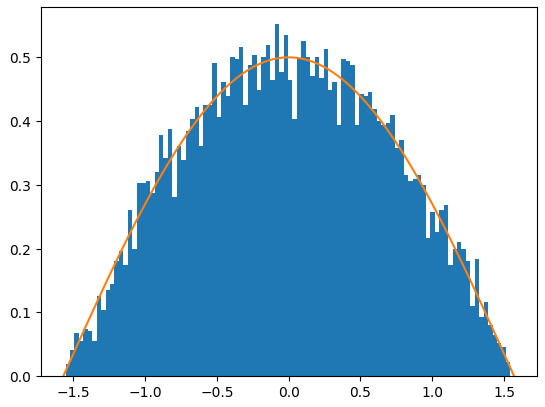
\includegraphics[width=0.5\textwidth]{figs/cos.png}
\caption{Code result and cosine distribution}\label{cosinedistribution}
\end{figure}

When making a prior set using bilby, we can use a cosine distribution provided in the package.

\begin{python}[Python3]
import numpy as np
import matplotlib.pyplot as plt
import bilby
priors = bilby.core.prior.PriorDict()
priors['dec'] = bilby.core.prior.Cosine(name = 'dec')
samples = priors.sample(10000)
plt.hist(samples['dec'], bins=100, density=True)
plt.plot(np.linspace(-np.pi/2, np.pi/2,100), 
         0.5*np.cos(np.linspace(-np.pi/2, np.pi/2,100)))
plt.show()
\end{python}

The result is almost same as Figure \ref{cosinedistribution}.

\end{example}

For more information, visit \href{https://en.wikipedia.org/wiki/Inverse_transform_sampling}{Wikipedia: Inverse Transform Sampling}.

\subsubsection{Confusion Matrix and ROC Curve}

The confusion matrix is used to evaluate the performance of the algorithm. It can be expressed as follows.

\begin{table}[h]
    \centering
    \begin{tabular}{c|cc}
         & Prediction: Positive & Prediction: Negative \\ \hline
        Actual result: Positive & True Positive (TP) & False Negative (FN)\\
        Actual result: Negative & False Positive (FP) & True Negative (TN)
    \end{tabular}
    \caption{Confusion Matrix}
    \label{confusion}
\end{table}

False positive rate(False alarm rate) is the proportion of data predicted as positive among data that are actually negative.

\begin{equation}
    \text{False positive rate} = \frac{\text{FP}}{\text{FP} + \text{TN}}
\end{equation}

Sensitivity(True positive rate) is the proportion of data that is actually positive, and the prediction result is also positive.

\begin{equation}
    \text{Sensitivity} = \frac{\text{TP}}{\text{TP} + \text{FN}}
\end{equation}

We can get the likelihood, accuracy, etc.. For more information about those, visit \href{https://en.wikipedia.org/wiki/Confusion_matrix}{Wikipedia - Confusion Matrix}.

Receive Operating Characteristic(ROC) curve is a plot that illustrates the performance of a binary classifier model at varying threshold values. The horizontal axis of the ROC curve is false positive rate, and the vertical axis is sensitivity.

The comparison curve is the $y=x$ straight line, which means that if the ROC curve is above $y=x$, the judgment was more correctly made than complete random classification, and if it is below, the classification was worse than complete random classification. For more information about those, visit \href{https://en.wikipedia.org/wiki/Receiver_operating_characteristic}{Wikipedia - Receive Operating Characteristic}.

\begin{figure}[h]
\centering
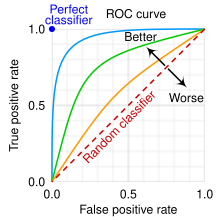
\includegraphics[width=0.5\textwidth]{figs/roc.png}
\caption{ROC curve - by Wikipedia}\label{roc}
\end{figure}
